\chapter{Estrategias de planificación de queries}
\label{cap:epq}

Decir por lotes

\section{Predicción de rendimiendo de transacciones de lectura}
\label{scheduling:prtl}
Lograr bajos tiempos de respuestas es uno de los objetivos principales en el diseño de un motor de búsqueda, ya que de esta forma se le puede entregar una respuesta oportunda al usuario. Además estos poseen acuerdos de nivel de servicio (SLA), por ejemplo, que el 99\% de las consultas sean respondidas en $100 ms$. Por lo tanto, las transacciones de lectura que requieren una gran cantidad de tiempo para ser resueltas degradan considerablemente la satisfacción del usuario, y es por esto que las máquinas de búsqueda están optimizadas para reducir el percentil más alto de los tiempos de respuesta (también llamado $tail latency$). Paralelizar el procesamiento de cada consulta es una solución promitente para reducir el tiempo de ejecución \citep{Jeon:2013, Tatikonda:2011}. Esto es posible con los modernos servidores que existen hoy en día que poseen múltiples núcleos, en donde se puede resolver una consulta paralelizando múltiples hilos de ejecución, reduciendo el tiempo de ejecución de esta.

Conocer de antemano la eficiencia de una \textit{query} es una ventaja muy importante, puesto que aquellas consultas que tomaran una mayor cantidad de tiempo en ser resueltas se les puede asignar un mayor número de \textit{threads} para procesarla, de esta manera se reduce el tiempo de procesamiento de las consultas y se cumple con la cota superior de tiempo prometida al usuario. Adicionalmente, que un sistema de recuperación de la información como un motor de búsqueda conozca anticipadamente cuánto tardará una consulta en ser procesada, permite implementar técnicas efectivas de planificación de transacciones de lecturas, por ejemplo, en el contexto de procesamiento paralelo de \textit{queries} por lotes (\textit{batches}) se pueden crear grupos de consultas que posean tiempos de respuesta parecidos, así se tiende a disminuir tanto el desbalance de carga entre los procesadores como el tiempo en procesar el \textit{batch} completo.

Existen trabajos en donde es estudia la correlación de algunos estadísticos presentes en las listas del índice invertido con el tiempo de respuesta de una transacción de lectura (citar trabajos que estudian los estadísticos). El más intuitivo es el número de documentos que hay en una lista invertida, mientras más larga es una lista invertida mayor es el tiempo que toma en ser resuelta. A continuación se presenta la implementación de métodos de predicción de eficiencia de queries basado en en los estudios (glasgow, sigir, oscar).  

\subsection{Método de predicción Glasgow}
\label{scheduling:glasgow}
El presente método \citep{Macdonald:2012} se basa en estadísticos obtenidos previamente calculados desde el índice invertido. Los puntajes de los documentos son obtenidos mediante el método BM25. Para cada consulta que llega al sistema, se toman los términos y para cada uno de ellos desde su propia lista invertida se obtiene los siguientes estadísticos $s(t)$:

\begin{list}{}{}
	\item \textbf{Media aritmética}. Se calcula la media aritmética del puntaje de los documentos.

	\item \textbf{Media geométrica}. Se calcula la media geométrica del puntaje de los documentos.

	\item \textbf{Media harmónica}.  Se calcula la media harmónica del puntaje de los documentos. 

	\item \textbf{Máximo puntaje}. Se obtiene el puntaje máximo perteneciente a algún documento dentro de la lista invertida. En otras palabras, se obtiene el \textit{upper bound} $UB_t$ de la lista. 

	\item \textbf{Varianza del puntaje}. Se extrae la varianza de puntaje de los documentos desde la lista invertida del término $t$. 
	
	\item \textbf{Número de documentos}. Se calcula el largo de la lista invertida. 

	\item \textbf{Número de maximos}. Se obtiene el número de veces en que aparece un puntaje máximo, es decir, el número de veces en que se actualiza el puntaje máximo. 

	\item \textbf{Número de documentos mayor a la media}. Se extrae el número de documentos que sobrepasa en puntaje al puntaje promedio. 
	
	\item \textbf{Número de documentos con puntaje máximo}. Se calcula el número de documentos que tienen el puntaje máximo dentro en la lista invertida del término $t$. 
	
	\item \textbf{Número de documentos dentro del 5\% más alto}. Se obtiene el número de documentos cuyos puntajes están dentro del 5\% superior dentrl de la lista invertida. 
	
	\item \textbf{Número de documentos dentro del 5\% del umbral (\textit{threshold})}. Se calcula el número de documentos cuyos puntaje están dentro del 5\% superior o inferior al umbral. Recordar que el \textit{threshold} es el puntaje de documento más bajo dentro del conjunto de los \textit{top-K}.
	
	\item \textbf{Número de inserciones en el conjunto de los mejores K documentos}. Para obtener este estadístico se asume que el término $t$ es una consulta con un solo término, se resuelve esta \textit{query} con el método \textit{Wand}  y se calcula el número de inserciones de documentos que se hizo al \textit{heap}. Recordar que las inserciones al \textit{heap} ocurren cuando el puntaje aproximado del documento supera el puntaje más bajo que en el \textit{heap} en ese momento (umbral o \textit{threshold}).
	
	\item \textbf{Frecuencia inversa de documento del término}. Se calcula el \textit{idf} del término $t$.
	
	\item \textbf{Tiempo en ser procesado el término}. Se obtiene el tiempo que toma ser procesado el término como una \textit{query} de un solo término.

\end{list}


Cada uno de los 14 estadísticos mencionados anteriormente están relacionados linealmente con la eficiencia de una transacción de lectura y son la base para la implementación del predictor, que está basado en un modelo de regresión lineal múltiple \citep{Chambers:1991}. A continuacion se muestra un resumen de estos estadísitcos en la Tabla \ref{tabla:estadisticosGlasgow}. 

\begin{table}[H]
\centering
\caption{Resumen de los estadísticos que se deben extraer desde el índice invertido}
\label{tabla:estadisticosGlasgow}
\begin{tabular}{|l|}
	\hline
	\textbf{Estadísticos del término s(t)} \\	
	1. Media aritmética	 \\ \hline
	2. Media geométrica	 \\ \hline
	3. Media harmónica	 \\ \hline
	4. Puntaje máximo	 \\ \hline
	5. Varianza del puntaje	 \\ \hline
	6. Número de documentos	 \\ \hline
	7. Número de máximos	 \\ \hline
	8. Número docs > media	 \\ \hline
	9. Número docs = máximo puntaje	 \\ \hline
	10. Número docs dentro del 5\% más alto	 \\ \hline
	11. Número docs dentro del 5\% del umbral	 \\ \hline
	12. Número de inserciones al conjunto top-K	 \\ \hline
	13. IDF	 \\ \hline
	14. Tiempo en resolver $t$ como \textit{query}	\\ \hline  
\end{tabular}
\end{table}


\subsection{Método de predicción SIGIR}
\label{scheduling:sigir}
En el contexto de un motor de búsqueda una consulta puede ser clasificada según el tiempo en que tome procesarla. En \citep{Jeon:2014} clasifican a una query como breve (0 - 30 ms), intermedia (30 - 80 ms) y prolongada ($ > 80 ms$). 


Al igual que el método anterior presentado en \ref{scheduling:glasgow}, se utilizan características de las listas invertidas de los términos de la consulta, es decir, toda la información necesaria estaba guardada en el índice invertido. En el presente método además se agregan características propias de las consultas que llegan al motor de búsqueda. 

// Hablar sobre el proceos de escritura y mostrar la tabla como resumen


Siguiendo la misma lógica del método presentado en la sección anterior, como las características presentadas en la Tabla \ref{tabla:estadisticosSigir} son de un solo término y generalmente las consultas contienen varios términos, se debe combinar estas características utilizando funciones de agregación. En este método se usa cuatro agregadores: máximo, mínimo, varianza y suma. Por ejemplo, para una query que contiene los términos 'casa' y 'perro', para cada una de las características de la Tabla \ref{tabla:estadisticosSigir} se calculará desde las dos listas invertidas el máximo, el mínimo, la varianza y la suma. Por lo tanto utilizando los agregadores para cada query se tiene 4 x 14 = 56 características totales.

Lo anterior es muy costoso mantenerlo en memoria RAM  obtenerlo a mano rápidamente y costoso calcularlo, se reduce la gamma de características.


Como se dijo anteriormente, en este nuevo método se agregarán características propias de la consulta. Estas características obtienen la complejidad de una transacción de lectura, la cual afecta el tiempo de ejecución de esta. Por ejemplo, el número de términos en la consulta y el idioma que está escrita, están correlacionado con el tiempo de ejecución. 

// resescritura incrementa la complejidad 

Las características propias de las queries son convenientes, ya que están disponible en tiempo de ejecución a un bajo costo. 


\begin{table}[!th]
\caption{Resumen de los estadísticos del presente método}
\begin{tabular}{|c|c|c|}
\hline
\textbf{Categoría} & \textbf{Característica} & \textbf{Descripción} \\ \hline
\multicolumn{ 1}{|p{3cm}|}{Característica} & MediaA & Media aritmética del puntaje \\ \cline{ 2- 3}
\multicolumn{ 1}{|p{3cm}|}{del} & MediaG & Media geométrica del puntaje \\ \cline{ 2- 3}
\multicolumn{ 1}{|p{3cm}|}{término} & MediaH & Media harmónica del puntaje \\ \cline{ 2- 3}
\multicolumn{ 1}{|c|}{} & MaxPuntaje & Puntaje máximo \\ \cline{ 2- 3}
\multicolumn{ 1}{|c|}{} & VarPuntaje & Varianza de puntaje \\ \cline{ 2- 3}
\multicolumn{ 1}{|c|}{} & Ndocs & Número de documentos \\ \cline{ 2- 3}
\multicolumn{ 1}{|c|}{} & Nmaxima & Número de máximos \\ \cline{ 2- 3}
\multicolumn{ 1}{|c|}{} & NdocsMedia & Número de documentos con puntaje mayor al puntaje medio \\ \cline{ 2- 3}
\multicolumn{ 1}{|c|}{} & NdocsMaximo & Número de documentos con puntaje máximo \\ \cline{ 2- 3}
\multicolumn{ 1}{|c|}{} & Ndocs5 & Número de documentos dentro del 5\% más alto \\ \cline{ 2- 3}
\multicolumn{ 1}{|c|}{} & NdocsThreshold & Número de documentos dentro del 5\% del umbral \\ \cline{ 2- 3}
\multicolumn{ 1}{|c|}{} & NdocsK & Número de inserciones al conjunto top-K \\ \cline{ 2- 3}
\multicolumn{ 1}{|c|}{} & IDF & Frecuencia Inversa de Documento \\ \cline{ 2- 3}
\multicolumn{ 1}{|c|}{} & timeTerm & Tiempo en resolver el término como una query \\ \hline
\multicolumn{ 1}{|p{3cm}|}{Característica} & Inglés & Indica si la consulta está en inglés o no \\ \cline{ 2- 3}
\multicolumn{ 1}{|p{3cm}|}{de la} & NumAumTerm & xxxxxx \\ \cline{ 2- 3}
\multicolumn{ 1}{|p{3cm}|}{consulta} & Complejidad & Indica el grado de complejidad de la consulta \\ \cline{ 2- 3} 
\multicolumn{ 1}{|c|}{} & Relax & Relax count applied or not \\ \cline{ 2- 3} 
\multicolumn{ 1}{|c|}{} & NumTermsAntes & Indica el número de términos en la consulta original \\ \cline{ 2- 3} 
\multicolumn{ 1}{|c|}{} & NumTermsDespues & Indica el número de términos después del proceso de reescritura \\ \cline{ 2- 3} 
\hline

\end{tabular}
\label{tabla:estadisticosSigir}
\end{table}


Tener las 56 características de cada uno de los términos del índice invertido en memoria es muy costoso para el sistema, sobretodo pensando en que ese mismo espacio (4.47 GB aproximadamente), se puede utilizar para guardar trozos del índice invertido (citar paper microsoft). Es por esto que se desarolla un estudio de las características más relevantes.

 



%Cuando un sistema está con una baja carga de trabajo paralelizar todas las consultas no tiene un impacto en el rendimiento, sin embargo, cuando un sistema está sometido a una moderada o %alta carga de trabajo paralelizar todas las queries entrantes es ineficiente, debido a que el costo de paralelizar queries cortas es alto.




\section{Wand \textit{multi-threaded}}
\label{scheduling:wm}
Dado que el método WAND \citep{Broder:2003} consiste es el método del estado del arte ocupado hoy en día por los motores de búsqueda, en esta investigación se asume un sistema que usa este método para obtener eficientemente los mejores K documentos a una transacción de lectura. Este algoritmo usa un \textit{ranking} basado en una evaluación de dos niveles. En el primer nivel, este usa una cota superior (\textit{upper bound}) al puntaje de cada documento para intentar descartarlos eficientemente. En el segundo nivel se computa el puntaje real de los documentos que pasa el primer nivel. Se utiliza una estructura de datos llamada \textit{heap} que va guardando el conjunto de los mejores K documentos hasta un determinado instante. El menor puntaje de este conjunto es usado como umbral (\textit{threshold}) para las evaluaciones del primer nivel, de esta forma se descarta rápidamente documentos que no pueden ser parte del conjunto final de los \textit{top-K} documentos. Esto permite un eficiente y a la vez seguro proceso de descarte que asegura que en el resultado final se encontrará el conjunto correcto y no se perderán documentos relevantes.

Existen dos formas de implementar Wand \textit{multithreaded}. Una de ellas es usando \textit{heaps} locales (LH), es decir, un \textit{heap} por hilo de ejecución (\textit{thread}) y el otro es usando \textit{heaps} compartidos (SH). El estudio en \citep{Rojas:2013} se muestra indicios que el esquema SH es generalmente más eficiente. Logrando rápidamente un óptimo valor para el threshold, el esquema SH posee las siguientes ventajas: (1) Se puede reducir el número de calculo de puntajes completos y (2) se ejecutan pocas operaciones de actualización del heap (reduciendo el número de \textit{locks} que se hace a la estructura de dato). A continuación se presenta el diseño llevado a cabo para ambos esquemas.

\subsection{Block max wand}
Recordar que en el método de Wand para descartar documentos y encontrar un documento que potencialmente podría estar en el conjunto \textit{top-K}, lo que se hace es usar los \textit{upper bounds} globales de cada lista, es decir, la máxima contribución (puntaje o \textit{score}) de algún documento de la lista invertida. Además, Wand tradicional es una estrategia DAAT, por lo que por cada lista invertida ocupa un puntero al documento actual que se desea evaluar. Además, usa un método que recibe como entrada un identificador del documento $docID$ y una lista invertida $L$, y retorna el primer $docID'$ que sea mayor o igual al documento $docID$. A esto se le conoce como movimiento de puntero profundo (\textit{deep pointer movement}) debido a la razón que generalmente implica una descompresión del boque en el que se encuentra el documento.

Sin embargo, como se dijo anteriormente en \ref{marco:bmw}, usando solo las máximas contribuciones por cada bloque no hará que el método funcione correctamente, puesto que hará que eventualmente se pierdan documentos que podrían estar en el conjunto final de los mejores $K$ documentos. Como ahora se tiene las máximas contribuciones por cada bloque, BMW utiliza otra función la cual recibe como parámetro un identificador de documento $docID$ y una lista invertida. Lo que se hace es mover el puntero actual al correspondiente bloque donde eventualmente se debería encontrar el documento $docID$. A esta función se le conoce como movimiento de puntero superficial (\textit{shallow pointer movement}), por la razón que no involucra una descompresión de bloque. Se debe notar que para que esta función trabaje correctamente se requiere tener almacenada las fronteras de cada uno de los bloques de las listas invertidas.

BMW utiliza dos principales ideas en su diseño: (1) Se usa los \textit{upper bounds} globales para determinar un pivote candidato (como en Wand tradicional), para luego usar los \textit{upper bounds} locales para determinar si es que el pivote candidato es un pivote real o no, y (2) Se intenta siempre utilizar \textit{shallow pointer movement} por sobre \textit{deep pointer movement}.

En el Algoritmo \ref{alg:bmw} se puede apreciar cómo el método \textit{Block-Max-Wand} trabaja. Recordar que todas las listas invertidas poseen un puntero al documento actual que se desea evaluar (\textit{currentDoc}). Lo primero que se hace es ordenar en orden creciente las listas invertidas de acuerdo a su correspondiente \textit{currentDoc}. La función \textit{findPivot()} es la misma que se utiliza en el método Wand tradicional (\ref{marco:wand}), se itera sobre las listas invertidas y se retorna la posición de la lista en donde se cumple que la suma de los \textit{upper bounds} globales es mayor al \textit{threshold} ($\theta$). Luego la función \textit{NextShallow()} se encarga de avanzar los punteros de las listas invertidas al inicio del bloque que debería contener el documento $d$. Posteriormente la función \textit{isRealPivot()} verifica si es que el pivote $p$ encontrado es un pivote real o no, para cada una de las listas desde la posición $0$ hasta la posición $p$, se suma los \textit{upper bounds} de los bloques en donde se encuentran los punteros (recordar que con \textit{NextShallow()} los punteros de las listas quedaron apuntando a los bloques en donde se debería encontrar el documento $d$), si la suma es mayor al threshold entonces retorna verdadero, de lo contrario retorna falso. El método \textit{scoreDoc()} calcula el puntaje del documento que se le pasa por parámetro. 

Cuando el método se da cuenta que $p$ no es un pivote real, lo que se hace es buscar un nuevo candidato a través de la función \textit{getNewCandidate()}, la cual hace avanzar los punteros de las listas invertidas hasta el bloque siguiente que contenga el mínimo $docID$. Para ver explicar de mejor manera esta idea se presenta la Figura \ref{fig:getNewCandidate}, aquí se puede ver que el documento $4868$ es el pivote, cuando este documento no es un pivote real (la función \textit{isRealPivote} retorna falso), lo que se hará es escoger un documento $d'$ tal que $d = min(d1,d2,d3,d4)$ en donde $d1,d2,d3$ son la frontera del bloque actual más uno (inicio del bloque siguiente) y $d4$ es el \textit{currentDoc} de la cuarta lista. Notar que para hacer un descarte seguro de documentos, siempre se debe incluir a la elección del nuevo candidato el \textit{currentDoc} de la lista inmediatamente siguiente a la lista pivote (en este caso 9009).  

\begin{figure}[!th]
\centering
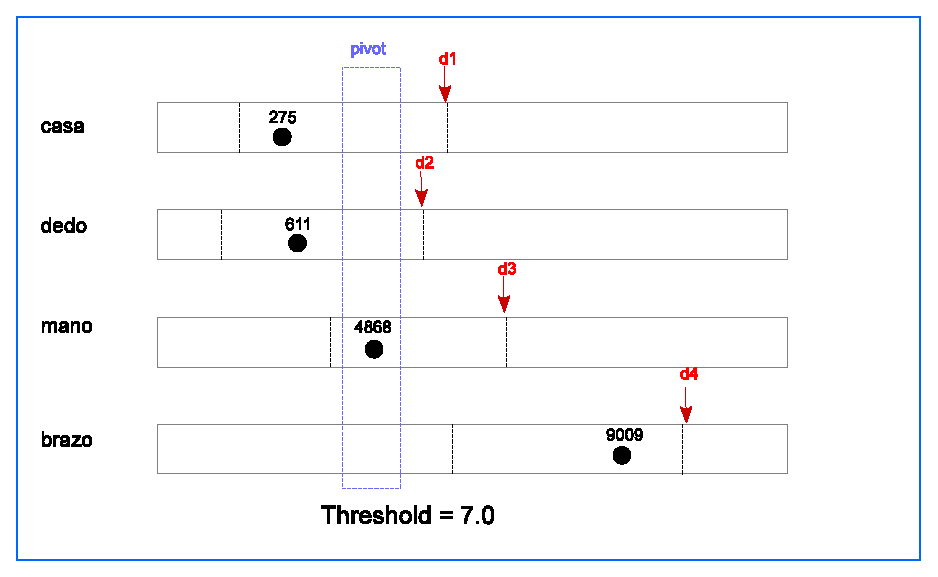
\includegraphics[scale=.75]{images/get_new_candidate.eps}
\caption{Ejemplo de cómo opera la functión getNewCandidate()}
\label{fig:getNewCandidate}
\end{figure}%y


\begin{algorithm}[!th]
\caption{\em $BMW(\theta, L, docID)$: Block Max Wand}
\label{alg:bmw}
\begin{algorithmic}[1]
\REQUIRE Un \textit{threshold} $\theta$, listas invertidas $L$ de los términos en la consulta
\ENSURE $docID$, si existe un documento $docID$ tal que $score(docID)$ $\geq$ $\theta$. de lo contrario END-OF-FILE
\WHILE {true}
	\STATE $Sort(L);$
	\STATE $p = findPivot(L,\theta);$
	\STATE $d = L[p] \rightarrow currentDoc;$
	\IF {$d == $ END-OF-FILE}
  		\STATE $break;$
	\ENDIF
		
	\FOR {$ i = 0...p $}
		\STATE $NextShallow(d, L[i]);$
	\ENDFOR
	
	\IF {$isRealPivot(\theta, p);$}
		\IF {$L[0] \rightarrow currentDoc == d$}
			\STATE $scoreDoc(d, p);$
			\FOR {$ i = 0...p $}
				\STATE $Next(d + 1, L[i]);$
			\ENDFOR
		\ELSE
			\WHILE {$List[p - 1] \rightarrow currentDoc == p $}
				\STATE $p = p - 1;$			
			\ENDWHILE
			
			\FOR {$ i = 0...p $}
				\STATE $Next(d, L[i]);$
			\ENDFOR
			
		\ENDIF		
	\ELSE	
		\STATE $d' = getNewCandidate();$
		\FOR {$ i = 0...p $}
			\STATE $Next(d', L[i]);$
		\ENDFOR
	\ENDIF
	
\ENDWHILE

\end{algorithmic}
\end{algorithm}

\subsection{Wand con heaps locales}
En el esquema LH, cada \textit{thread} procesa una porción del índice invertido mientras mantiene un \textit{heap} local con los mejores $K$ documentos que el específico hilo de ejecución ha encontrado hasta ahora. Al final del proceso, los resultados deben ser reunido en un solo conjunto final global. Los resultados en \citep{Rojas:2013} muestran que el esquema LH es más eficientes para aquellas transacciones que toman poco tiempo en ser resueltas. En la Figura \ref{fig:wand-heap-local} se muestra el esquema de ejecución para \textit{heaps} locales explicado anteriormente. 

\begin{figure}[!ht]
\centering
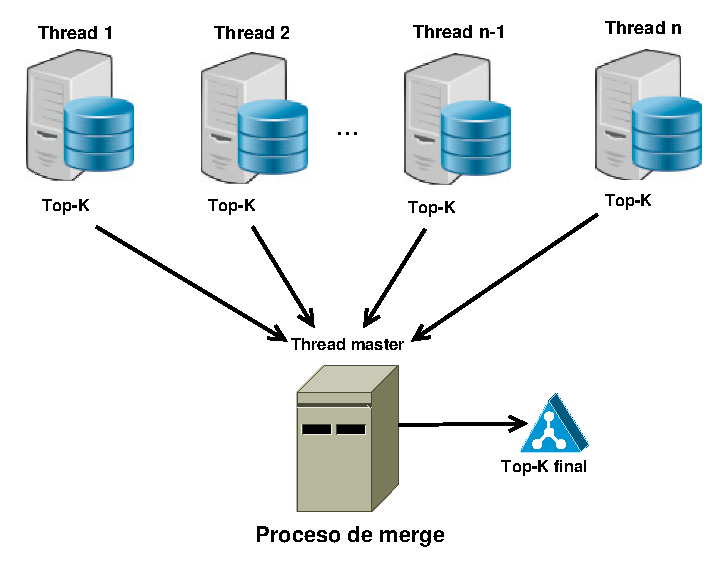
\includegraphics[scale=.75]{images/wand_heaps_locales.eps}
\caption{Esquema de ejecución de algoritmo WAND con heaps locales}
\label{fig:wand-heap-local}
\end{figure}

El diseño aplicado para implementar el esquema LH se puede ver en la Figura \ref{fig:TopKMultiThreadWandOperatorLocal}. La clase principal es la TopKMultiThreadWandOperatorLocal, que es la encargada de controlar el paralelismo en la resolución de las transacciones. Para explicar de mejor manera cada una de las clases involucradas en la implementación, se presenta el siguiente diccionario de datos.

\begin{figure}[!ht]
\centering
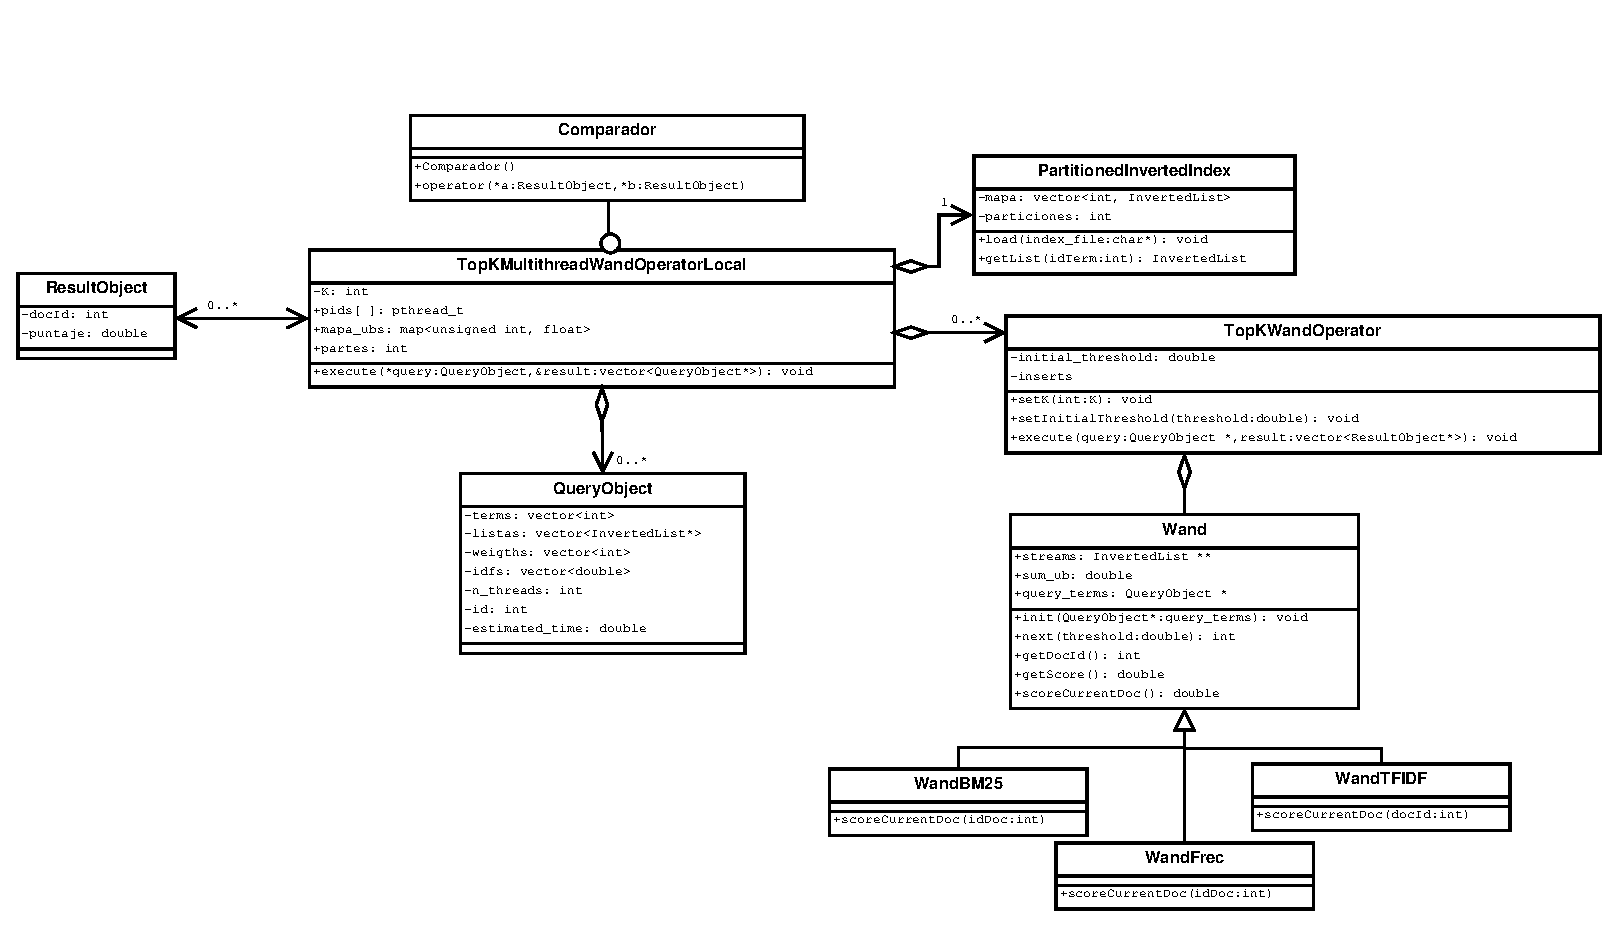
\includegraphics[scale=.75]{images/TopKMultiThreadWandOperatorLocal.eps}
\caption{Diagrama de clases para el esquema LH}
\label{fig:TopKMultiThreadWandOperatorLocal}
\end{figure}

\begin{list}{}{}
	\item \textbf{TopKMultiThreadWandOperatorLocal}. Clase encargada de devolver los mejores K documentos para una query dada. Si es que la query debe ser resuelta en forma paralela, esta clase además debe controlar el paralelismo que se produce en la resolución de ésta, inicializando las variables correspondientes para lanzar los hilos de ejecución y luego escogiendo los mejores documentos desde todos los heaps creados por los diferentes threads (proceso de merge). En esta clase se define un mapa que asocia cada término del índice invertido con el puntaje del mejor documento en esa lista invertida (upper bound de la lista invertida) y además se define cuántos documentos se van a retornar al final del proceso (atributo K). El método execute inicializa las variables locales para los diferentes threads, posteriormente hace el llamado al método \emph{thread-execute} (en el cual se llevará a cabo la resolución de la transacción de lectura en forma paralela), finalmente se toman los resultados parciales de cada uno de los hilos de ejecución y se ejecuta el proceso que mezcla los resultados, retornando solo los mejores K documentos. 
	
	\item \textbf{PartitionedInvertedIndex}. Clase que tiene la tarea de almacenar el índice invertido y extraer desde aquí las listas invertidas de documentos para cada uno de los términos de las transacciones de lectura. El almacenamiento el índice se lleva a cabo mediante un mapa cada término su lista invertida correspondiente y para la extracción de estas listas se usa el método getList.
	
	\item \textbf{TopKWandOperator}.  Cada thread tendrá su propio objeto TopKWandOperator encargado de obtener los mejores K documentos. El cálculo de este conjunto se realiza en el método execute con la ayuda de un objeto de tipo Wand asociado.
	
	\item \textbf{Wand}. Clase que controla la lógica del algoritmo wand. Lleva a cabo el proceso de inserción de documentos en el heap y todo lo que esto conlleva. Existen diferentes tipos de objetos Wand que se pueden utilizar, entre ellos están WandBM25, WandFrec y WandTFIDF, donde la única diferencia entre ellos es el método de que calcula el puntaje de cada documento. Por ejemplo, WandBM25 utiliza BM25 (citar) y WandTFIDF utiliza tf-idf (citar también). 
	
	\item \textbf{ResultObject}. Clase que se utiliza para guardar los mejores K documentos.
	
	\item \textbf{QueryObject}. Clase que representa una transacción de lectura. Está constutuída sus términos,  las respectivas listas invertidas y pesos de cada uno de ellos, la cantidad de threads con los cuales se resolverá dicha transacción y el tiempo estimado de procesamiento (este tiempo se predice al momento de resolver la query).

\end{list}




\subsection{Wand con heap compartido}
\label{scheduling:whc}
En el esquema SH cada thread procesa una porción del índice. Sin embargo, ahora un solo heap es creado y accedido por todos los threads. En este caso no se requiere de mezclar los resultados y el proceso de descarte tiende a ser más eficiente porque los documentos con mayor puntaje tienden a estar en el heap. Acceder al heap debe ser controlado por un lock o algún método similar que garantice el acceso exclusivo de los threads al heap. Este esquema es más eficiente que el LH en queries que toman mayor tiempo en ser resueltas.

El diseño implementado para este esquema posee como clase principal a TopKMultiThreadWandOperatorLocks y difiere del modelo implementado para el esquema LH en el sentido que ahora se debe controlar el acceso concurrente a los datos compartidos como el heap y el threshold. A continuación se presenta el diccionario de datos del esquema SH mostrado en la Figura \ref{fig:TopKMultiThreadWandOperatorLocks}.

\begin{figure}[!ht]
\centering
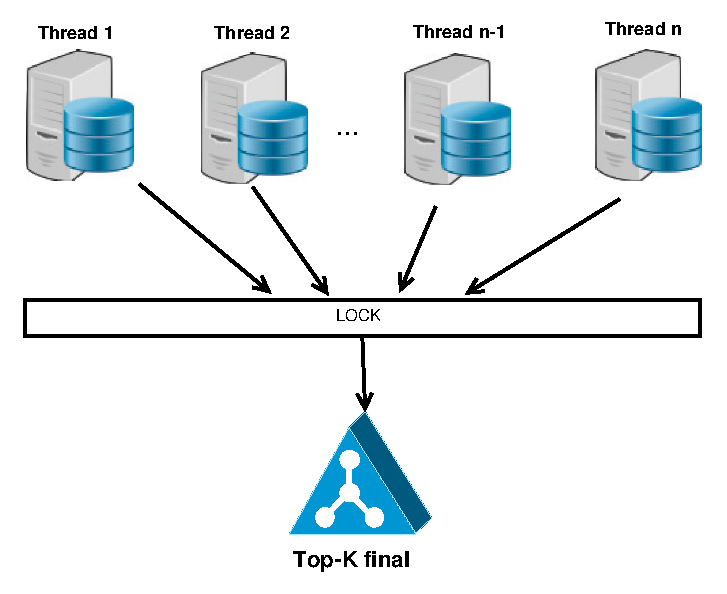
\includegraphics[scale=.75]{images/wand_heaps_compartido.eps}
\caption{Esquema de ejecución de algoritmo WAND con heap compartido}
\label{fig:wand-heap-compartido}
\end{figure}

\begin{list}{}{}
	\item \textbf{TopKMultiThreadWandOperatorLocks}. Clase encargada de inicializar las variables compartidas y de lanzar los threads requeridos para procesar la transacción de lectura.
	
	\item \textbf{WandThreadData}. Clase anidada a TopKMultiThreadWandOperatorLocks que contendrá todas las variables compartidas para el procesamiento de las consultas. Dentro de los atributos más importantes destaca el mutex utilizado para controlar el acceso al heap compartido y además al threshold (en este esquema es un threshold global y compartido a todos los threads).
	
	\item \textbf{Wand}. Al igual que en el esquema anterior, esta clase se encarga de llevar a cabo el proceso de inserción de documentos en el heap y de las actualizaciones del threshold. El método scoreCurrentDoc es el encargado de entregarle un puntaje a cada documento y dependerá de qué tipo de Wand se este utilizando (BM25, WandFrec, WandTFIDF). 

	\item \textbf{PartitionedInvertedIndex}. Clase encargada de almacenar el índice invertido. Posee un método llamado getList que recibe como parámetro el identificador de un documento y retorna la lista invertida asociada. 

\end{list}

\begin{figure}[!ht]
\centering
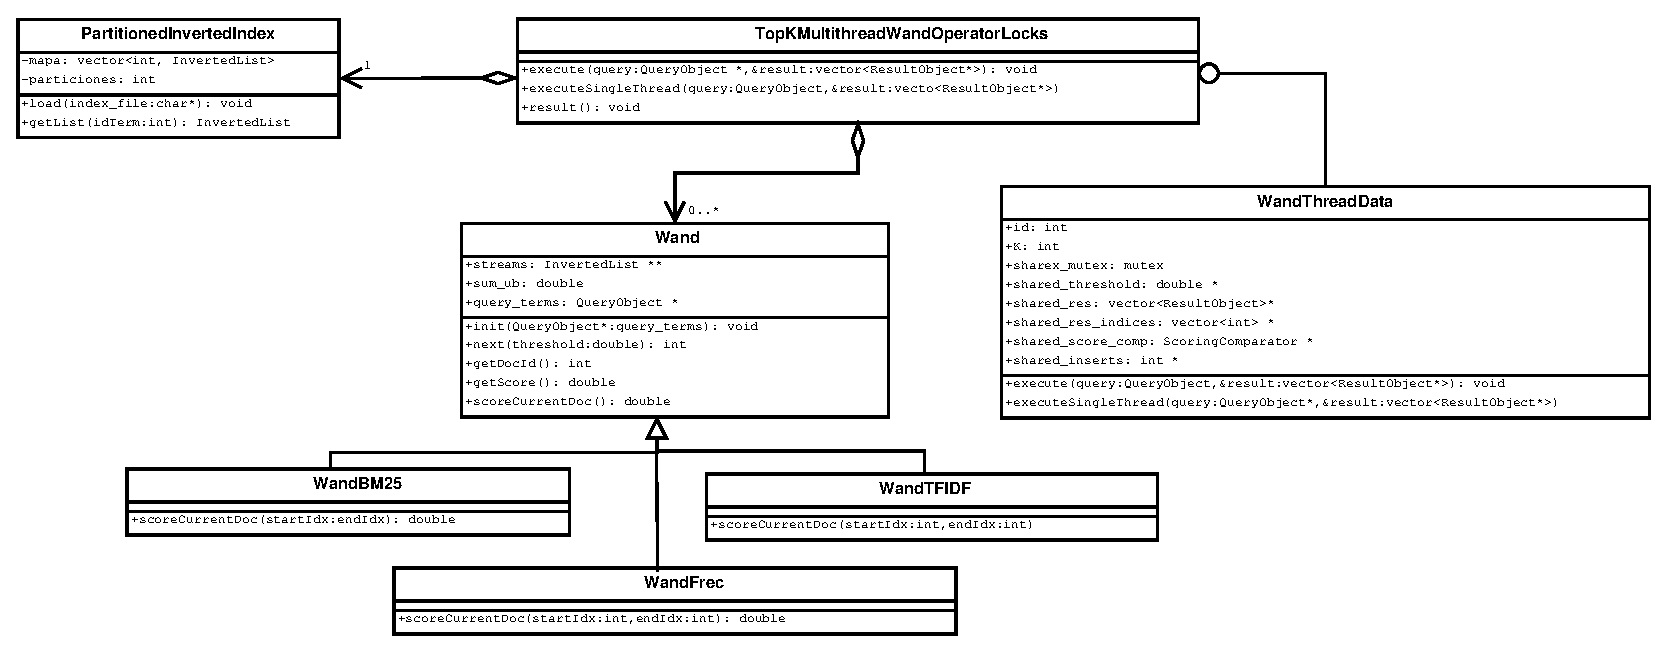
\includegraphics[scale=.75]{images/TopKMultiThreadWandOperatorLocks.eps}
\caption{Diagrama de clases para el esquema SH}
\label{fig:TopKMultiThreadWandOperatorLocks}
\end{figure}




\section{Estrategias de planificación}
\label{scheduling:es}

Nosotros optamos por un enfoque de Wand Heap Compartido para ser usado en los experimentos.

Se habla de enfoque de bloques también.

\subsection{Estrategia \textit{1TQ}}
\label{scheduling:baseline}
Un simple camino para construir un sistema que responda a múltiples consultas simultáneamente usando múltiple hilos de ejecución, es usando estos hilos de manera independiente. Para hacer esto se debe mantener un conjunto de \textit{threads} consumidores que trabajarán en paralelo y se encargarán de resolver las \textit{queries} secuencialmente (una a una) desde una misma cola, esto es lo que en este trabajo se denomina estrategia de Un Thread Por Query (1TQ). En la Figura \ref{fig:1TQ} se puede apreciar el esquema de ejecución en donde cada uno de los procesos genera una petición de alguna consulta en la cola, si quedan \textit{queries} por procesar entonces se le asigna al proceso una consulta que tendrá que resolver de manera secuencial. Se debe tener en cuenta que cada vez que un proceso genera una solicitud de \textit{query}, se bloquea la estructura de datos que contiene las consultas a procesar y luego se procesa la solicitud, de esta forma se asegura un acceso seguro por parte de los distintos \textit{threads}. 

\begin{figure}[H]
\centering
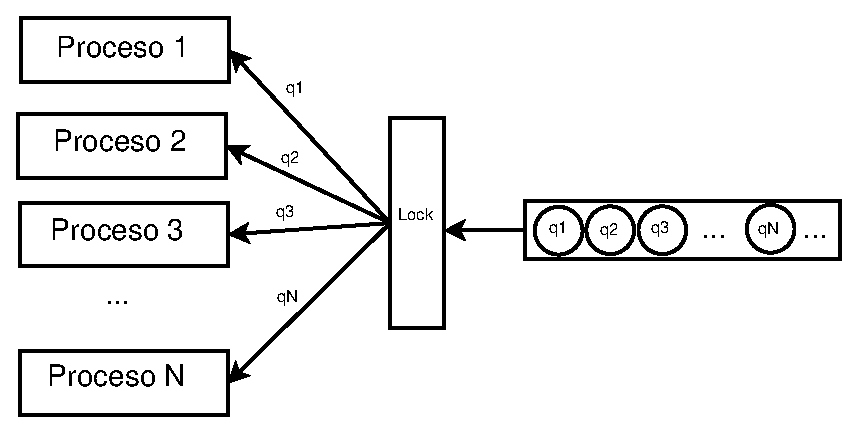
\includegraphics[scale=.75]{images/1TQ.eps}
\caption{Ejemplo de procesamiento estrategia 1TQ}
\label{fig:1TQ}
\end{figure}

Este esquema tiene la ventaja que es simple y fácil de implementar y controlar. Sin embargo, existen sistemas de recuperación de la información como los motores de búsqueda verticales que cuando están ejecutando \textit{batches} de \textit{queries} deben parar su ejecución porque transacciones de escritura han llegado al sistema, y este deben actualizar la información del índice invertido. Solo después de la fase de actualización el sistema es capaz de ejecutar el siguiente \textit{batch} de transacciones de lectura. Al final de cada conjunto de consultas, es posible que algunos hilos de ejecución del sistema finalicen su trabajo y que no tengan más \textit{queries} para procesar, por lo que ellos tienen que esperar que los \textit{threads} restantes finalicen su trabajo antes que el sistema entre en la fase de actualización de su índice invertido o bien, se pase a la ejecución del siguiente \textit{batch} de consultas.
Sin embargo, aunque cada hilo de ejecución está secuencialmente ejecutando una transacción de lectura diferente, algunas de estas operaciones puede tomar un tiempo cosiderable, de esta forma se produce una importante pérdida de eficiencia, aunque la intuición nos dice que esto se puede mitigar con \textit{queries} que requieran poca cantidad de tiempo para ser procesada (trabajos pequeños o \textit{small jobs}). 
En la Figura \ref{fig:small_jobs} queda reflejado lo dicho en el párrafo anterior. Si los trabajos que cada \textit{thread} está ejecutando son pequeños, entonces probablemente la pérdida de trabajo al final de cada \textit{batch} de consultas será menor al trabajo que se pierde cuando los trabajos son grandes (ver Figura \ref{fig:large_jobs}).  


\begin{figure}[H]
\centering
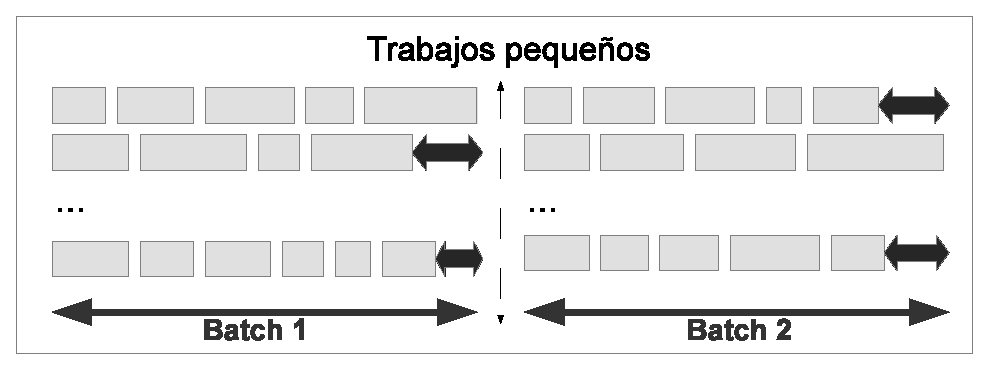
\includegraphics[scale=.75]{images/small_jobs.eps}
\caption{Ejecución en paralelo de \textit{small jobs}}
\label{fig:small_jobs}
\end{figure}

\begin{figure}[H]
\centering
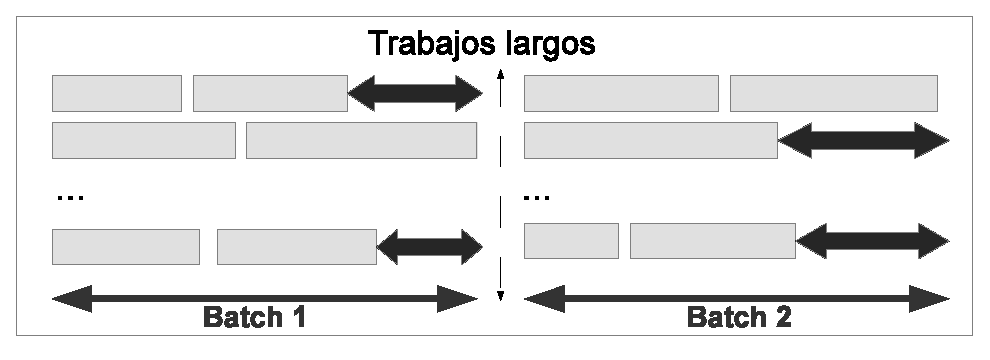
\includegraphics[scale=.75]{images/large_jobs.eps}
\caption{Ejecución en paralelo de \textit{large jobs}}
\label{fig:large_jobs}
\end{figure}



\subsection{Estrategia unidades de trabajo}
\label{scheduling:unidadestrabajo}
Con respecto a los esquemas explicados hasta ahora, el esquema 1TQ tiene la ventaja que no solo requiere menos control, sino que también permite a los hilos de ejecución trabajar sin pausa mientras un \textit{batch} de consultas está siendo procesado. En esta sección se propone un esquema híbrido basado en unidades de procesamiento (\textit{Processing Units}) que aproveche las ventajas de ambos enfoques. (se requiere ver el tema de bloques).
En este nuevo esquema de planificación, las consultas pasan a través de una fase en la cual cada \textit{query} es evaluada y se determina un apropiado número de unidades de procesamiento (\textit{processing units}) para poder resolver dicha consulta. Este proceso es llevado a cabo de manera similar al proceso en donde se determina la cantidad de \textit{threads} apropiados para resolver una determina transacción de lectura. Este número de unidades de procesamiento es creado y asociado a cada consulta, finalmente se guarda en una cola de unidades de trabajo. Un conjunto de \textit{threads} consumidores extraen las unidades desde la cola y las procesa independientemente. Cuando un \textit{thread} finalice el procesamiento de la unidad de trabajo actual automáticamente leerá la siguiente unidad de trabajo desde la cola. 
Generalmente lo que se hace habitualmente es estimar el número de \textit{threads} con el que se resolverá la consulta, como se muestra en la Figura \ref{fig:unit_process} en este nuevo enfoque se intenta estimar el número de unidades de trabajo con el que se resolverá cada consulta. Además, se debe controlar el acceso concurrente de los hilos de ejecución a la cola de unidades de trabajo, de tal manera que solo un thread tenga acceso exclusivo a la estructura de datos. 

\begin{figure}[!th]
\centering
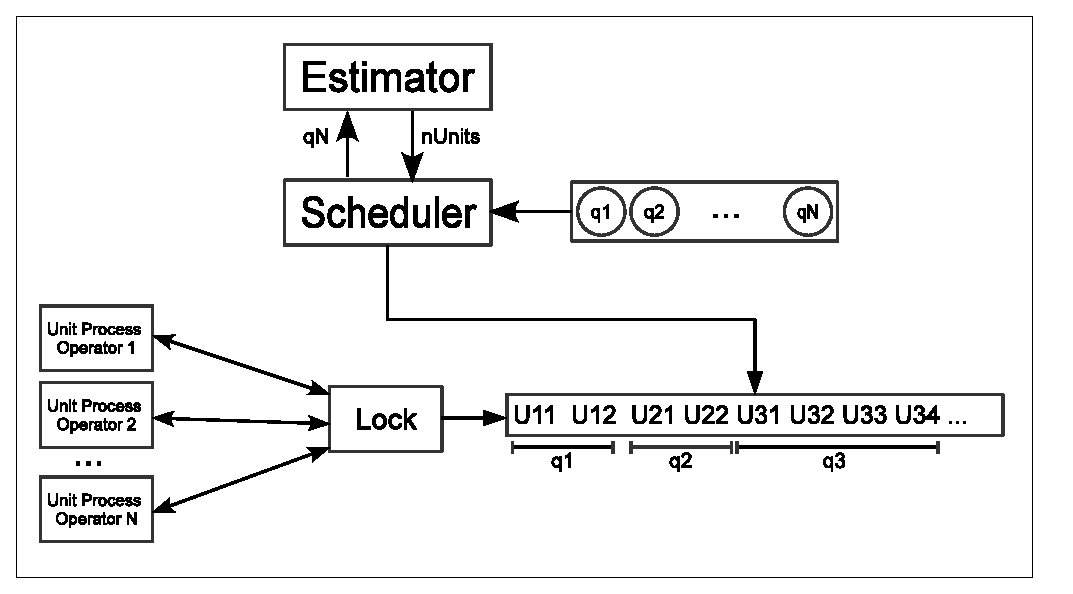
\includegraphics[scale=.75]{images/unit_process.eps}
\caption{Procesamiento de consultas utilizando unidades de trabajo}
\label{fig:unit_process}
\end{figure}

El procesamiento de cada hilo de ejecución es una versión de Wand con heap compartido (SH), adaptado de manera tal que cada unidad de trabajo es resuelta independientemente de si existen otras unidades siendo procesada al mismo tiempo o no. La única excepción es que la unidad que inicializa la consulta es siempre ejecutada antes del resto de las otras unidades de la misma consulta y la entrega de resultados se hace una vez que todas las unidades de trabajo de la \textit{query} han finalizado. Este enfoque híbrido permite reducir el tiempo perdido al final de cada \textit{batch} sin generar una importante pérdida de trabajo mientras las \textit{queries} del \textit{batch} están siendo procesadas.


\subsection{Estrategia FR}
\label{scheduling:fr}

// Se explica

// Esquema de ejecución

// Algoritmo

// Ejemplo de cómo van quedando los bloques


